
\section{Feature Evaluation}

The success on classification depends on the predictive value of the features
posses. Therefore, it is necessary asses whether a feature is useful in the
discrimination between formal and informal housing. The evaluation requires the
satellite image to be divided into the formal and informal classes. This division
is represented using a ground truth; this is a mask covering the satellite image
indicating where the informal areas are located.

The mask is used to divide each block of pixels into the two classes: formal or
informal. Each block has a vector of features, characterizing that particular
block. Because blocks of the same class are grouped together, the features
associated with the same class are grouped together as well. This allows for
the analysis of the distribution of the features in both classes. If the
distribution of a certain feature varies substantially between the two classes,
this indicates as a suitable candidate for classification of informal regions.

The groundtruth mask is constructed using a vector file containing the
boundaries of informal areas. The boundary file is rasterized and applied on
top of the satellite image, creating a mask of the location of the informal
housing areas.  Because classification and feature calculation is performed on
blocks instead of pixels, the pixel based mask transformed into a block based
mask. In this block based mask, every pixel represents a block where zero
represents formal and one represents informal. This effectively creates
a ground truth of informal areas in the satellite image.  

The predictive value of a feature can be visualized using a boxplot of the two
classes. When a feature is distinctive on its own, the distribution of the
values in the two classes will be different. The data used for the evaluation
comes from three small sections of the image. As priorly mentioned, this
creates a more even division of classes which should provide a more accurate
evaluation of the selected feature.

% TODO: make sure numbers here are valid
The features will be calculated for all combinations of image sections, color
bands, block sizes, and scales. This resulted in large amounts of data, of
which only a selection will be shown in the following sections. For both HoG
and LSR, the features are extracted from the three sections presented in Figure
\ref{fig:sections} on all the three color bands. To analyze the impact of the
block size and scale parameters, block sizes 20, 40 and 60 will be used in
combination with scales 50, 100, 150 and 200. The block sizes will be combined
together with the scales, resulting in a large number of combinations of
parameters.  Some combinations, however, are not valid, e.g when the scale is
smaller than the block size, and will therefore be omitted. The individual
impact of each of the two parameters, is evaluated by the use of a comparison
between the baseline and the increased parameter. This is, for example,
a comparison between the results obtained from a block size of 20 compared to
a block size of 60, with all other parameters constant. 

Because every combination of image section, block size and scale will have
three different results due to the RGB color bands, we refrain from visualizing
all bands and pick the first band, which is red. The results do actually vary
a bit between the red, green, and blue band, but it is not significant enough
to explicitly visualize all three versions of the results. Furthermore, only
a single feature for each extraction method is shown to reduce the number of
plots.

\subsection{Histogram of Oriented Gradients}

\begin{figure}
\begin{tabular}{cc}
  \subfloat{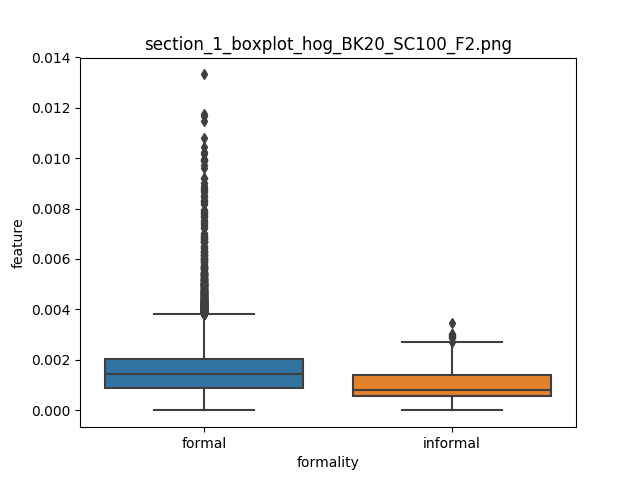
\includegraphics[width=4cm]{images/HoG/inc_bk/section_1_boxplot_hog_BK20_SC100_F2}}&
  \subfloat{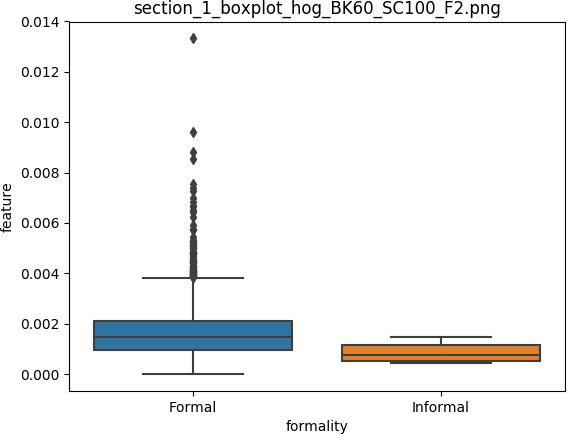
\includegraphics[width=4cm]{images/HoG/inc_bk/section_1_boxplot_hog_BK60_SC100_F2}}\\ 
  \subfloat{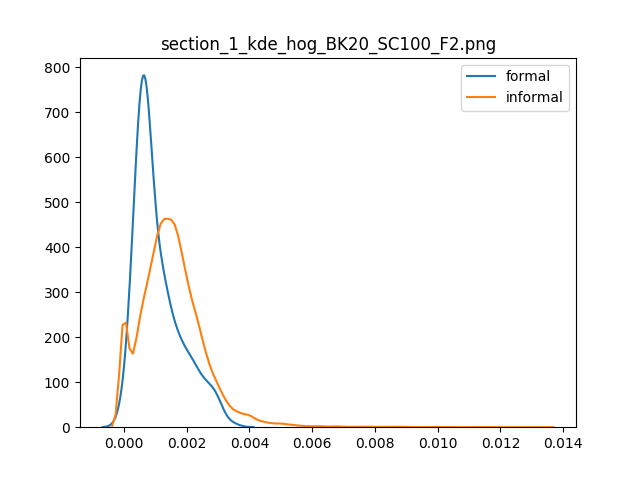
\includegraphics[width=4cm]{images/HoG/inc_bk/section_1_kde_hog_BK20_SC100_F2}}&
  \subfloat{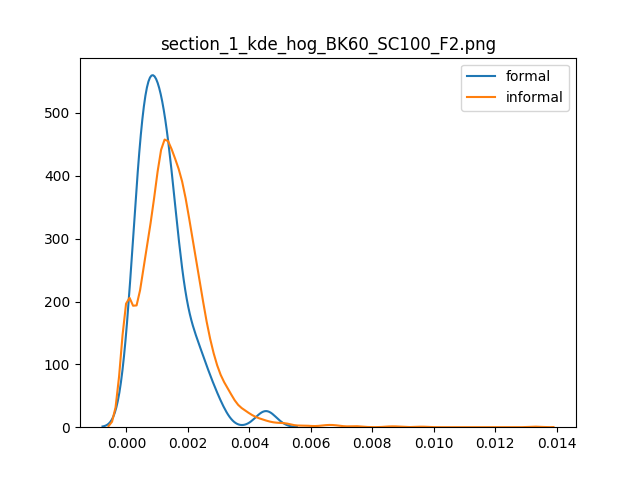
\includegraphics[width=4cm]{images/HoG/inc_bk/section_1_kde_hog_BK60_SC100_F2}}
\end{tabular}
\caption{The effect of increased block size on the HoG features. From left to
right: a block size of 20 and 60 respectively.}
\label{hog_inc_bk}
\end{figure}

For the HoG, the third feature is selected for visualization in this section.
This feature best illustrated the difference in distribution. Figure
\ref{hog_inc_bk} shows the effect of an increased block size on the
distribution of values in both classes. This example uses a constant scale of
100 pixels and a variable block size of 20 and 60 pixels. The experiment with
a block size of 40 is performed as well, but is ommited from the figure to keep
the results brief. A more comprehensive visualization of the evaluation can be
found in the appendix. It seems that the block size, in this case, does not
influence the both distrutions significantly. As a result an increase in the
size of a block should have little to no influence on the predictive value of
the feature.

\begin{figure}
\begin{tabular}{cc}
  \subfloat{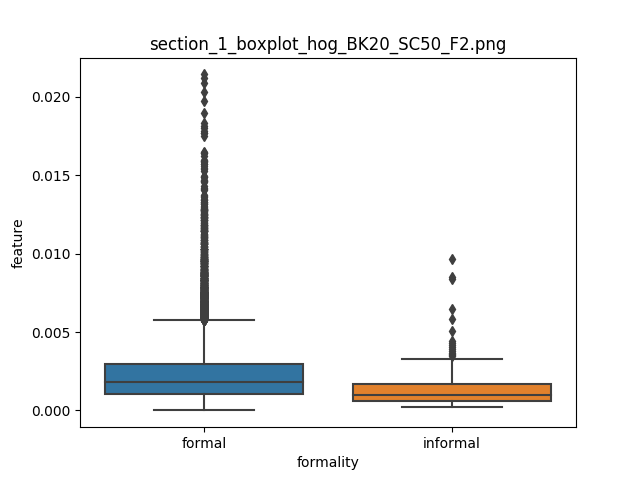
\includegraphics[width=4cm]{images/HoG/inc_sc/section_1_boxplot_hog_BK20_SC50_F2}}&
  \subfloat{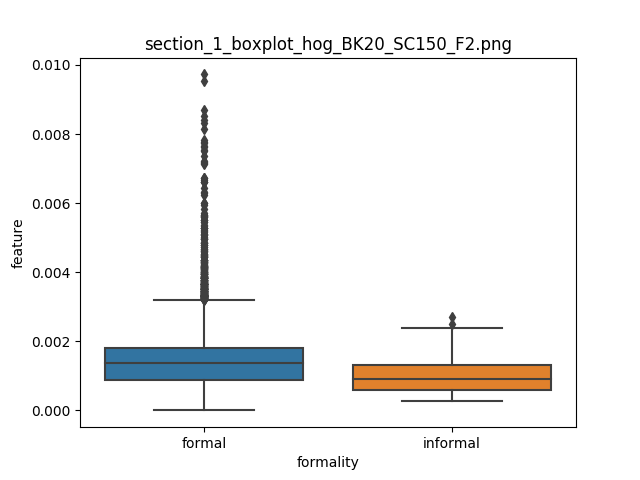
\includegraphics[width=4cm]{images/HoG/inc_sc/section_1_boxplot_hog_BK20_SC150_F2}}\\
  \subfloat{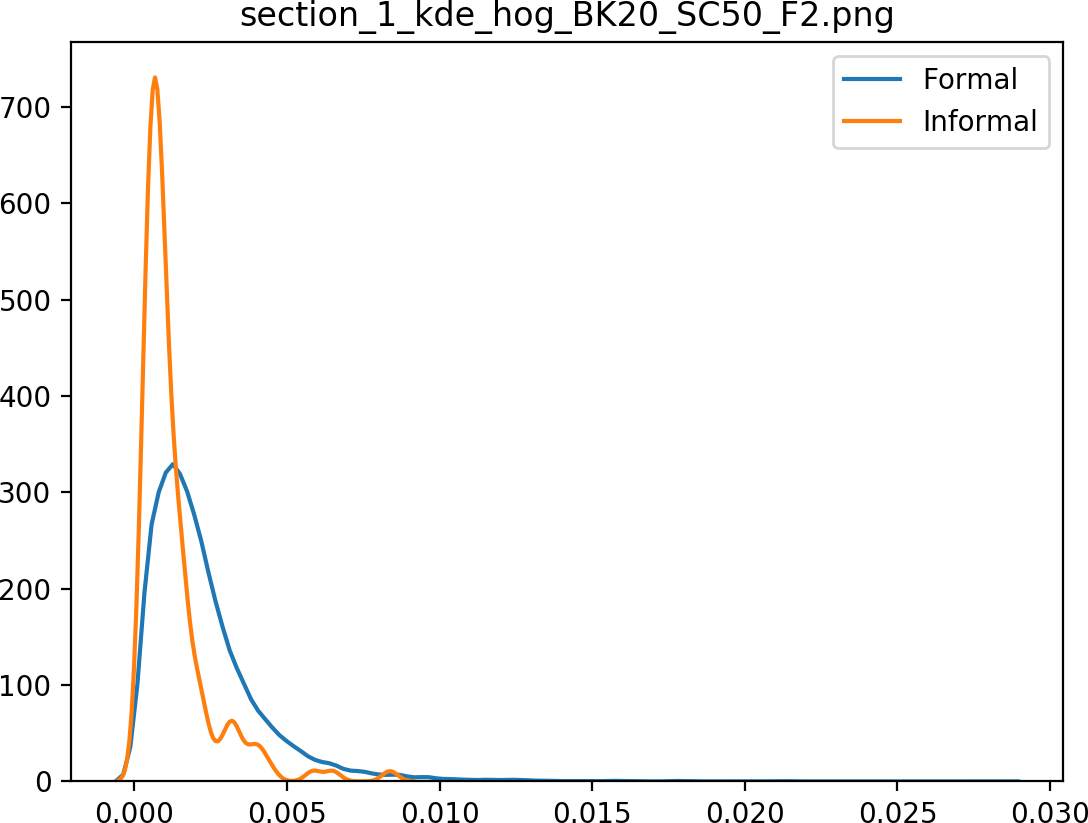
\includegraphics[width=4cm]{images/HoG/inc_sc/section_1_kde_hog_BK20_SC50_F2}}&
  \subfloat{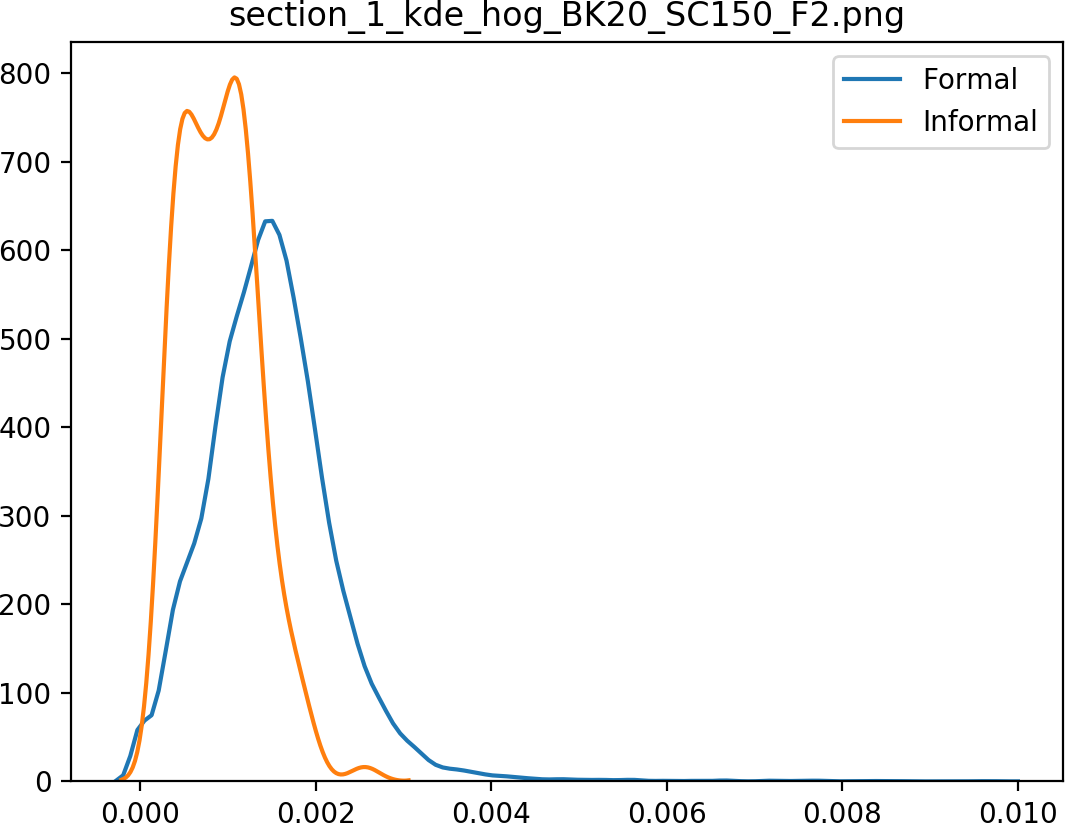
\includegraphics[width=4cm]{images/HoG/inc_sc/section_1_kde_hog_BK20_SC150_F2}}\\
\end{tabular}
\caption{The effect of increased scale on the HoG features. From left to
right: a scale of 50 and 150 respectively}
\label{hog_inc_sc}
\end{figure}

Figure \ref{hog_inc_sc} illustrates the effect of increased scale on a constant
block size. It seems to indicate that an increased scale leads to an increased
separatation of the two distribution, thus increasing the predictiveness of the
feature. Scales larger than 150 do not seem to improve the performance. In
contrast, the performance actually seems to decrease with scales larger than
150. Therefore, for the HoG features, the scale of 150 is used in all further
experiments 

% TODO: explain why this happens?

\subsection{Line Support Region}

The most distinctive feature of LSR was chosen for visualization, in this case,
it was the second feature. The second feature is the mean, which seems to work
quite well. The mean of the first section is visualized in since this section
produced the most distinct results from the three sections. Similar to the
analysis of HoG, the increase of the block size does not influence the
distribution of the two classes. The difference is as neglible as displayed in
the comparison of the HoG in Figure \ref{hog_inc_bk}

%\begin{figure}
%\begin{tabular}{cc}
%  \subfloat{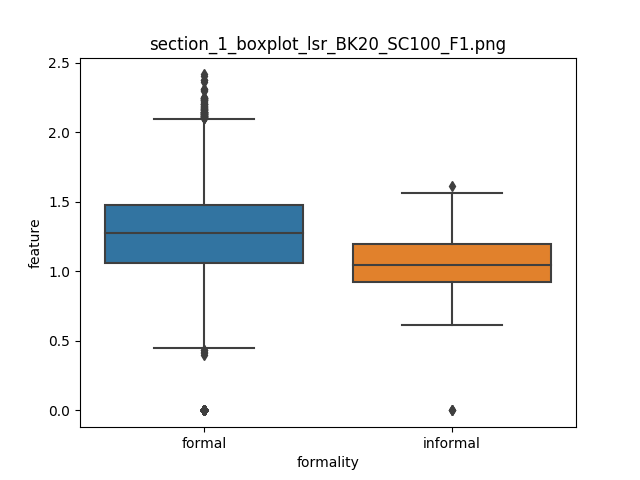
\includegraphics[width=4cm]{images/LSR/inc_bk/s1/section_1_boxplot_lsr_BK20_SC100_F1}}&
%  \subfloat{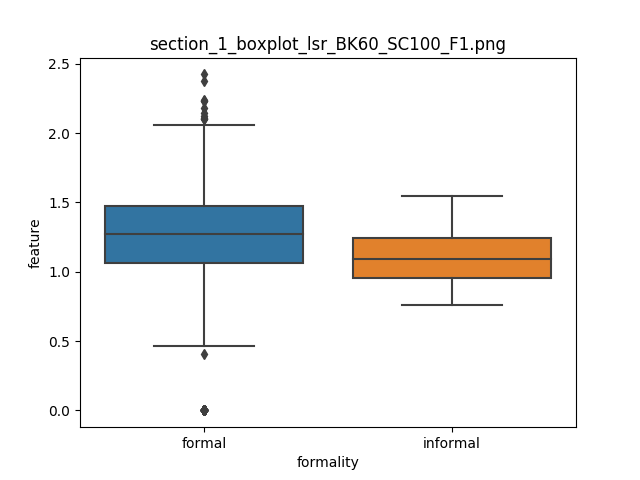
\includegraphics[width=4cm]{images/LSR/inc_bk/s1/section_1_boxplot_lsr_BK60_SC100_F1}}\\
%  \subfloat{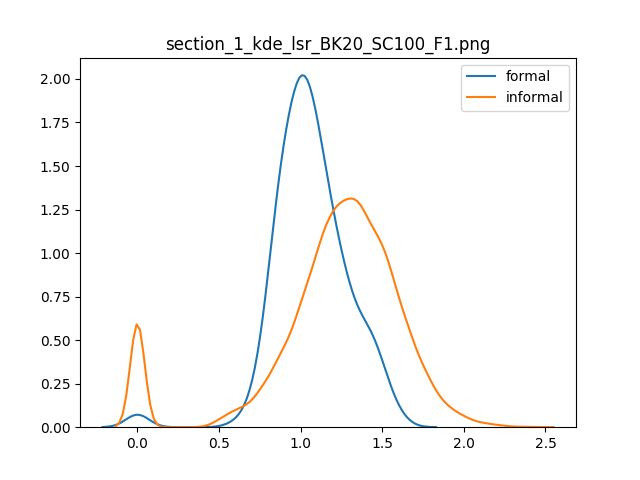
\includegraphics[width=4cm]{images/LSR/inc_bk/s1/section_1_kde_lsr_BK20_SC100_F1}}&
%  \subfloat{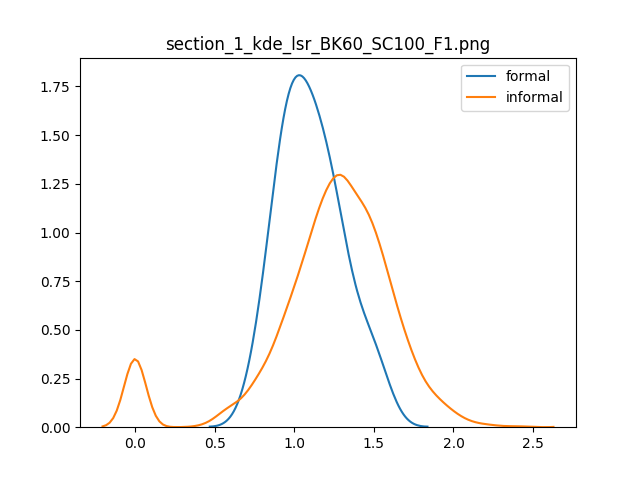
\includegraphics[width=4cm]{images/LSR/inc_bk/s1/section_1_kde_lsr_BK60_SC100_F1}}
%\end{tabular}
%\caption{The effect of increased block size on the second SLR feature. From left to
%right: a block size of 20 and 60 respectively.}
%\label{lsr_inc_bk}
%\end{figure}

\begin{figure}
\begin{tabular}{cc}
  \subfloat{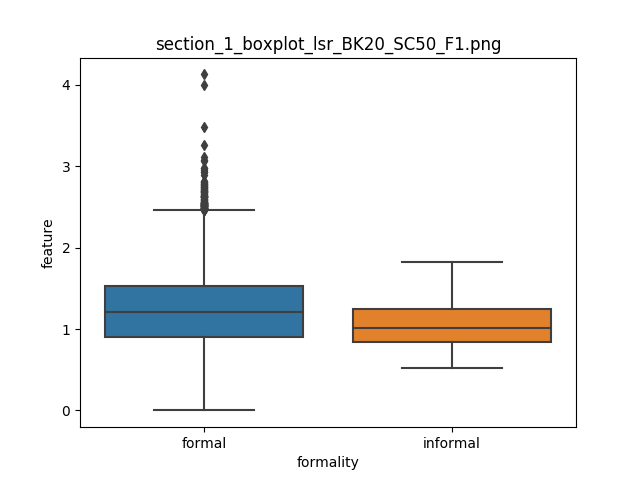
\includegraphics[width=4cm]{images/LSR/inc_sc/s1/section_1_boxplot_lsr_BK20_SC50_F1}}&
  \subfloat{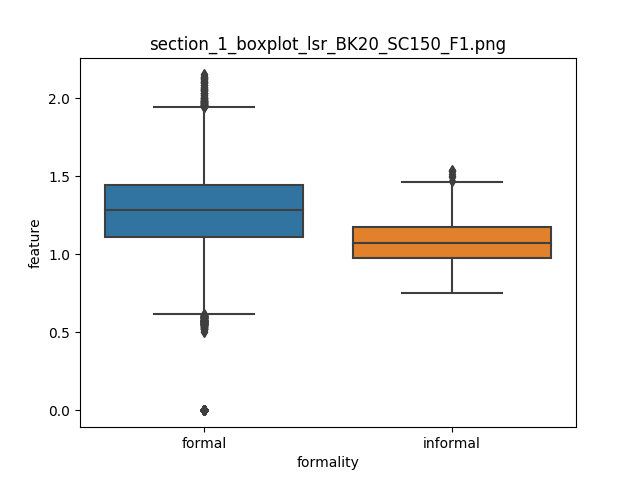
\includegraphics[width=4cm]{images/LSR/inc_sc/s1/section_1_boxplot_lsr_BK20_SC150_F1}}\\
  \subfloat{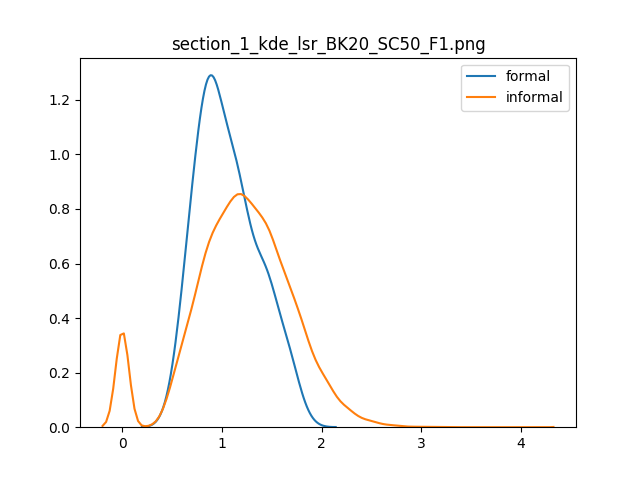
\includegraphics[width=4cm]{images/LSR/inc_sc/s1/section_1_kde_lsr_BK20_SC50_F1}}&
  \subfloat{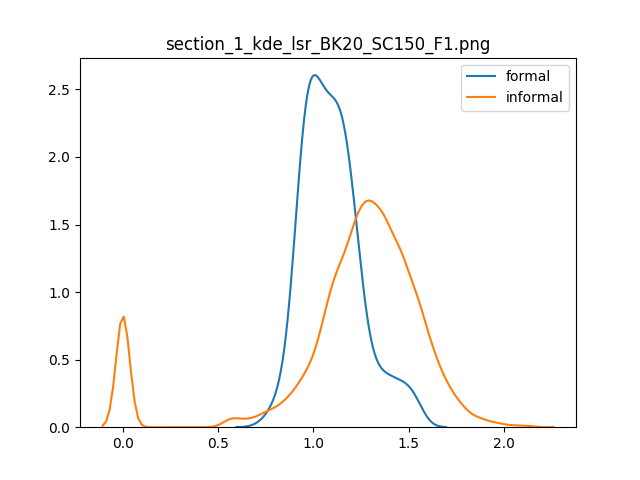
\includegraphics[width=4cm]{images/LSR/inc_sc/s1/section_1_kde_lsr_BK20_SC150_F1}}
\end{tabular}
\caption{The effect of increased scale on the second SLR feature. From left to
right: a scale of 50 and 150 respectively.}
\label{lsr_inc_sc}
\end{figure}

An increase in scale of the LSR feature is visualized in Figure
\ref{lsr_inc_sc}. Similar to the Histogram of Oriented gradients, it appears
that an increase in scale seems to increase the difference between the
distributions of the formal and informal classes.  However, the the clear
division between distrubutions does not translate to the other two sections. In
section 2 the distributions are somewhat distinct. Section 3 has barely any
distinction between the two distributions. The use of the other LSR features
together with the two different color bands does not seem to help.  It might be
that the features of LSR fail to produce correct results in areas with
vegetation, which section 2 and 3 both posess. The difference in vegetation can
be seen in Figure \ref{fig:sections} where the image sections are displayed.


\subsection{Road Intersection Density}

% The evaluation of the road density features is different than the HoG and LSR
% features. 

\subsection{Conclusion}

% TODO: make sure numbers are valid
It seems that, in general, an increase in scale improves the distinctness of
the two classes. However, increasing the scale is computationally very
expensive. Just on these smaller subsections, the time to compute features at
a high scale is measured in hours rather than minutes. Using features with high
scales on large images would therefore not be feasable. Besides, increasing the
scale gives diminishing returns while taking significantly more time to
compute. For the smaller sections, higher scales, such as 200 or 250 is
used, but on large scale images this is brought down to a managable 150.

With the right parameters, there is a clear distinction between the two classes
for both the HoG and LSR features. Therefore, we conclude that these features
can be used classification. 

% Conclude the usefullness of the features


